\documentclass[12pt]{book}
\usepackage{fontspec}
\setmainfont{TeX Gyre Pagella}
\usepackage[paperwidth=8in,paperheight=8in,margin=0.6in]{geometry}
\usepackage{xcolor}
\usepackage{amssymb}
\usepackage{tikz}
\usetikzlibrary{arrows.meta}
\pagestyle{empty}
\setlength{\parindent}{0pt}

\newcommand{\artnote}[1]{{\color{gray!70}\small\itshape [Illustration: #1]}\par\vspace{0.3in}}
\newcommand{\bigline}[1]{{\Huge #1}\par}
\newcommand{\pagenum}[1]{\vfill{\color{gray!50}\footnotesize #1}}
\newcommand{\sprollpage}{\newpage\vspace*{0.4in}}
\newcommand{\threeshapes}[3]{%
\begin{tikzpicture}
\draw[line width=2.5pt, #1] (-1.3,0) circle (0.32in);
\draw[#2] (-0.15,-0.3) -- (0.15,0.3) -- (0.45,-0.3) -- cycle;
\draw[line width=2.5pt, #3] (0.9,-0.3) rectangle (1.5,0.3);
\end{tikzpicture}}

\begin{document}

% ============ FRONT COVER ============
\thispagestyle{empty}
\begin{center}
\vspace*{1.1in}
{\Huge \textbf{SPROLL 01}}\\[0.4in]
{\huge \textbf{Something Happened}}\\[0.5in]
\threeshapes{black}{fill=orange!60}{black}
\\[0.5in]
{\large \textit{the first Pop}}\\[0.3in]
{\small The Sproll Curriculum $\cdot$ Cycle I: Pops}
\end{center}

% ============ PAGE 2: half-title / indicia ============
\sprollpage
\begin{center}
\vspace*{1.5in}
{\Large The Sproll Curriculum}\\[0.2in]
{\normalsize Cycle I --- Pops: Things, Differences, and Counting}\\[0.6in]
{\small Sproll 01 of 40 \quad $\cdot$ \quad follows Sproll 00: A Difference}
\end{center}
\pagenum{2}

% ============ PAGE 3 ============
\sprollpage
\begin{center}
\vspace*{0.6in}
\artnote{a circle, a triangle, and a square, evenly spaced, all drawn the same plain black outline, none highlighted, none connected -- an open field around them}
\threeshapes{black}{draw=black, fill=none, line width=2.5pt}{black}
\vspace{0.4in}
\bigline{There are three ways to go.}
\end{center}
\pagenum{3}

% ============ PAGE 4 ============
\sprollpage
\begin{center}
\vspace*{0.6in}
\artnote{the same three shapes, unchanged, with a small open hand or a gentle dotted circle hovering near them, inviting a choice -- nothing selected yet}
\threeshapes{black}{draw=black, fill=none, line width=2.5pt}{black}
\vspace{0.2in}
{\color{gray!60}\Large (a hand hovers, deciding)}
\vspace{0.3in}
\bigline{Choose one.}
\end{center}
\pagenum{4}

% ============ PAGE 5 ============
\sprollpage
\begin{center}
\vspace*{0.6in}
\artnote{the same three shapes, but now the square is drawn solid and bold while the circle and triangle are faded to a light gray outline}

\begin{tikzpicture}
\draw[line width=1.5pt, gray!45] (-1.3,0) circle (0.32in);
\draw[gray!45, line width=1.5pt] (-0.15,-0.3) -- (0.15,0.3) -- (0.45,-0.3) -- cycle;
\draw[line width=3.5pt, black, fill=black!10] (0.9,-0.3) rectangle (1.5,0.3);
\end{tikzpicture}
\vspace{0.4in}
\bigline{You chose the square.}
\end{center}
\pagenum{5}

% ============ PAGE 6 ============
\sprollpage
\begin{center}
\vspace*{0.5in}
\artnote{the same faded circle and triangle, the same bold square, now with a small clean label sitting just above the square}
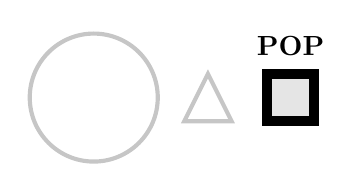
\begin{tikzpicture}
\draw[line width=1.5pt, gray!45] (-1.3,0) circle (0.32in);
\draw[gray!45, line width=1.5pt] (-0.15,-0.3) -- (0.15,0.3) -- (0.45,-0.3) -- cycle;
\draw[line width=3.5pt, black, fill=black!10] (0.9,-0.3) rectangle (1.5,0.3);
\node at (1.2,0.65) {\bfseries POP};
\end{tikzpicture}
\vspace{0.3in}
\bigline{That choice is a Pop.}
\end{center}
\pagenum{6}

% ============ PAGE 7 ============
\sprollpage
\begin{center}
\vspace*{0.6in}
\artnote{the original three plain, unhighlighted shapes from page 3, exactly as they first appeared, side by side}
\threeshapes{black}{draw=black, fill=none, line width=2.5pt}{black}
\vspace{0.4in}
\bigline{Before, there were three ways to go.}
\end{center}
\pagenum{7}

% ============ PAGE 8 ============
\sprollpage
\begin{center}
\vspace*{0.6in}
\artnote{the three shapes with a single bold arrow sweeping from the group toward the square, suggesting a single decisive motion}
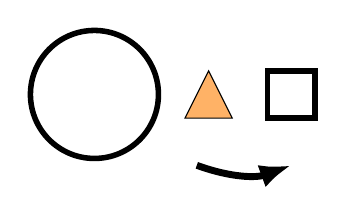
\begin{tikzpicture}
\draw[line width=2pt] (-1.3,0) circle (0.32in);
\draw[fill=orange!60] (-0.15,-0.3) -- (0.15,0.3) -- (0.45,-0.3) -- cycle;
\draw[line width=2pt] (0.9,-0.3) rectangle (1.5,0.3);
\draw[-{Latex[length=4mm]}, line width=2.5pt] (0,-0.9) to[bend right=20] (1.2,-0.9);
\end{tikzpicture}
\vspace{0.4in}
\bigline{Then something happened.}
\end{center}
\pagenum{8}

% ============ PAGE 9 ============
\sprollpage
\begin{center}
\vspace*{0.6in}
\artnote{a small horizontal ledger strip, like a single line in a notebook, with one square drawn inside it -- the first entry in a history}
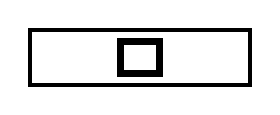
\begin{tikzpicture}
\draw[line width=1.5pt] (-1.4,-0.35) rectangle (1.4,0.35);
\draw[line width=2.5pt] (-0.25,-0.2) rectangle (0.25,0.2);
\end{tikzpicture}
\vspace{0.4in}
\bigline{Now we have a history.}
\end{center}
\pagenum{9}

% ============ PAGE 10 ============
\sprollpage
\begin{center}
\vspace*{0.6in}
\artnote{a fresh, unmarked circle, triangle, and square, exactly like page 3 -- a clean restart}
\threeshapes{black}{draw=black, fill=none, line width=2.5pt}{black}
\vspace{0.4in}
\bigline{Let's try again.}
\end{center}
\pagenum{10}

% ============ PAGE 11 ============
\sprollpage
\begin{center}
\vspace*{0.6in}
\artnote{the same three shapes, but now the triangle is bold and solid while the circle and square are faded}

\begin{tikzpicture}
\draw[line width=1.5pt, gray!45] (-1.3,0) circle (0.32in);
\draw[fill=orange!60, line width=3.5pt] (-0.15,-0.3) -- (0.15,0.3) -- (0.45,-0.3) -- cycle;
\draw[line width=1.5pt, gray!45] (0.9,-0.3) rectangle (1.5,0.3);
\end{tikzpicture}
\vspace{0.4in}
\bigline{This time, choose the triangle.}
\end{center}
\pagenum{11}

% ============ PAGE 12 ============
\sprollpage
\begin{center}
\vspace*{0.5in}
\artnote{two small ledger strips stacked one above the other -- the top strip contains a square, the bottom strip contains a triangle, each clearly separate}
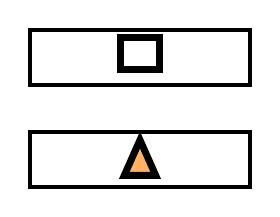
\begin{tikzpicture}
\draw[line width=1.5pt] (-1.4,0.55) rectangle (1.4,1.25);
\draw[line width=2.5pt] (-0.25,0.75) rectangle (0.25,1.15);
\draw[line width=1.5pt] (-1.4,-0.75) rectangle (1.4,-0.05);
\draw[fill=orange!60, line width=2.5pt] (-0.2,-0.6) -- (0,-0.15) -- (0.2,-0.6) -- cycle;
\end{tikzpicture}
\vspace{0.3in}
\bigline{Now there are two histories.}
\end{center}
\pagenum{12}

% ============ PAGE 13 ============
\sprollpage
\begin{center}
\vspace*{0.5in}
\artnote{a new field of three plain unlabeled shapes -- circle, triangle, square -- with the circle now shown bold and solid, the triangle and square faded, exactly as the choosing convention was established earlier in this book}

\begin{tikzpicture}
\draw[line width=3.5pt, black, fill=black!10] (-1.3,0) circle (0.32in);
\draw[gray!45, line width=1.5pt] (-0.15+0.9,-0.3) -- (0.15+0.9,0.3) -- (0.45+0.9,-0.3) -- cycle;
\draw[line width=1.5pt, gray!45] (2.1,-0.3) rectangle (2.7,0.3);
\end{tikzpicture}
\vspace{0.3in}
\bigline{You chose the circle.}\vspace{0.1in}
{\Large Pop $\bigcirc$.}
\end{center}
\pagenum{13}

% ============ PAGE 14 ============
\sprollpage
\begin{center}
\vspace*{0.5in}
\artnote{a second, different field of three shapes, drawn solid/filled this time to show they are a new and different set of options from the first field -- a filled circle, a filled triangle, a filled square -- with the triangle shown bold and the other two faded}

\begin{tikzpicture}
\draw[line width=1.5pt, gray!45, fill=gray!15] (-1.3,0) circle (0.32in);
\draw[fill=orange!60, line width=3.5pt] (-0.15+0.9,-0.3) -- (0.15+0.9,0.3) -- (0.45+0.9,-0.3) -- cycle;
\draw[line width=1.5pt, gray!45, fill=gray!15] (2.1,-0.3) rectangle (2.7,0.3);
\end{tikzpicture}
\vspace{0.3in}
\bigline{A new field. You chose the triangle.}\vspace{0.1in}
{\Large Pop $\blacktriangle$.}
\end{center}
\pagenum{14}

% ============ PAGE 15 (closing / hand-off) ============
\sprollpage
\begin{center}
\vspace*{0.3in}
\artnote{a two-line ledger strip: the first line contains a small circle labeled Pop, the second line contains a small filled triangle labeled Pop, stacked so both committed choices are visible together as one growing history}
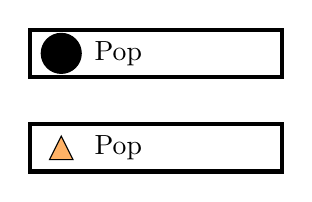
\begin{tikzpicture}
\draw[line width=1.5pt] (-1.6,0.5) rectangle (1.6,1.1);
\filldraw[fill=black] (-1.2,0.8) circle (0.1in);
\node[right] at (-0.9,0.8) {Pop};
\draw[line width=1.5pt] (-1.6,-0.7) rectangle (1.6,-0.1);
\draw[fill=orange!60] (-1.35,-0.55) -- (-1.2,-0.25) -- (-1.05,-0.55) -- cycle;
\node[right] at (-0.9,-0.4) {Pop};
\end{tikzpicture}
\vspace{0.2in}
\bigline{How many Pops happened?}\vspace{0.15in}
{\Huge \textbf{Two Pops happened.}}
\vspace{0.35in}\\
{\small \textit{--- turn the page for Sproll 02: What Happened First? ---}}
\end{center}
\pagenum{15}

% ============ PAGE 16: Note for Grown-Ups (backmatter) ============
\sprollpage
\vspace*{0.3in}
{\large \textbf{A Note for Grown-Ups}}
\vspace{0.2in}

\normalsize
This book introduces the first formal move of the series: a Pop. A Pop is not a shape, a mark, or an object. It is the act of choosing one thing from several things that could have happened, so that afterward there is a history rather than only a set of possibilities.

\vspace{0.15in}
Sproll 00 asked what can be distinguished. This book asks what happens when a distinction is chosen. That is a real difference, not a rephrasing: distinguishing does not by itself remove any of the other possibilities, but choosing does. Before the choice, there were three ways to go. After it, one history exists, and the other two ways of going stayed unchosen.

\vspace{0.15in}
The book deliberately repeats the choosing experiment with a different outcome (page 11) so a child can see that the same starting possibilities can lead to different, equally legitimate histories. Nothing about the circle, triangle, or square determined which would be chosen; the choosing is what made the history.

\vspace{0.15in}
Counting is introduced here as a count of Pops within a single growing history, not a count of objects that happen to be sitting on the page, and not two objects simply appearing. If a history is written H = $\langle e_1, e_2, \ldots, e_n \rangle$, its length $|H| = n$ is exactly what this book teaches a child to find by counting committed choices. This is deliberately narrower than saying a number is a property of a history in general; it says only that a finite history's length can be counted. Much later, the curriculum can let a child notice that ``two'' shows up in many different structures built from the four primitives, such as two objects, two events, two available continuations, two bound components, or two equivalence classes, and let the abstraction of ``two'' emerge from what stays invariant across those cases, rather than asserting the generalization here.

\vspace{0.3in}
{\small Sproll 02: What Happened First? continues directly from this book's final page.}
\pagenum{16}

\end{document}
